\documentclass[a4paper,10pt]{article}
\usepackage[left=3cm,top=3cm,right=3cm,bottom=3cm,head=4cm,includefoot]{geometry}

%%%%%%%%%%%%%%%%%%%%%%%%%%%%%%%%%%%%%%%%%%%%%%%%%%%%%%%%%%%%%%%%%%%%%%%%
% Paquetes utilizados
%%%%%%%%%%%%%%%%%%%%%%%%%%%%%%%%%%%%%%%%%%%%%%%%%%%%%%%%%%%%%%%%%%%%%%%%

% Graficos complejos
\usepackage{graphicx}
\usepackage{rotating}
\usepackage{caption}
\usepackage{subcaption}
\usepackage{placeins}

% Soporte para el lenguaje español
\usepackage{textcomp}
\usepackage[utf8]{inputenc}
\usepackage[T1]{fontenc}
\DeclareUnicodeCharacter{B0}{\textdegree}
\usepackage[spanish]{babel}

% Codigo fuente embebido
\usepackage{listings}

% PDFs embebidos para el apendice
\usepackage{pdfpages}

% Matematicos
\usepackage{amssymb,amsmath}

% Tablas complejas
\usepackage{multirow}

% Formato de parrafo
\setlength{\parskip}{1ex plus 0.5ex minus 0.2ex}

%%%%%%%%%%%%%%%%%%%%%%%%%%%%%%%%%%%%%%%%%%%%%%%%%%%%%%%%%%%%%%%%%%%%%%%%
% Titulo
%%%%%%%%%%%%%%%%%%%%%%%%%%%%%%%%%%%%%%%%%%%%%%%%%%%%%%%%%%%%%%%%%%%%%%%%

% Titulo principal del documento.
\title{\textbf{Trabajo Practico 1: ConcuCalesita}}

% Informacion sobre los autores.
\author{\\
  Arana Andrés, \textit{P. 86.203}                                 \\
  \texttt{and2arana@gmail.com}                                     \\ [2.5ex]
  Arias Damián, \textit{P. 89.952}                                 \\
  \texttt{arias.damian@gmail.com}                                  \\ [2.5ex]
  Sergio Matias Piano, \textit{P. 85.191}                          \\
  \texttt{smpiano@gmail.com}                                       \\ [2.5ex]
                                                                   \\
  \normalsize{2do. Cuatrimestre de 2014}                           \\
  \normalsize{75.59 Técnicas de Programación Concurrente 1}        \\
  \normalsize{Facultad de Ingenieria, Universidad de Buenos Aires} \\
}
\date{}

%%%%%%%%%%%%%%%%%%%%%%%%%%%%%%%%%%%%%%%%%%%%%%%%%%%%%%%%%%%%%%%%%%%%%%%%
% Documento
%%%%%%%%%%%%%%%%%%%%%%%%%%%%%%%%%%%%%%%%%%%%%%%%%%%%%%%%%%%%%%%%%%%%%%%%

\begin{document}

% ----------------------------------------------------------------------
% Top matter
% ----------------------------------------------------------------------
\thispagestyle{empty}
\maketitle

\begin{abstract}

  Este informe sumariza el desarrollo del trabajo practico 1 de la materia Técnicas de Programación Concurrente I (75.59) dictada en el segundo cuatrimestre de 2014 en la Facultad de Ingenieria de la Universidad de Buenos Aires. El mismo consiste en la construccion de una simulación del uso de una calesita utilizando técnicas de sincronización de procesos.

\end{abstract}

\clearpage

% ----------------------------------------------------------------------
% Indice
% ----------------------------------------------------------------------
\tableofcontents
\clearpage


% ----------------------------------------------------------------------
% Desarrollo
% ----------------------------------------------------------------------
%\part{parte}


\section{Análisis del problema}

\subsection{Descripción}

El sistema deberá contar con la posibilidad de simular la llegada de los niños del barrio a la calesita del parque. A medida que van llegando, estos se irán encolando en la ventanilla única para comprar un boleto.

En ventanilla estará presente el cajero quien desacolará al primero de la fila, le cobrará el valor del boleto y pasará a atender al siguiente niño.
El dinero recaudado es guardado en la caja, teniendo acceso exclusivo el cajero mientras la esté usando.
Cada cierto tiempo vendrá el auditor a controlar la recaudación tomando el control momentaneamente de la caja.

Los niños que hayan comprado el boleto se dirigirán a la cola de entrada de la calesita donde aguardarán su turno para ingresar.
La calesita tiene una capacidad fija y no empieza la vuelta hasta que estén todos sus lugares completos.
Cuando termina una vuelta los niños que estaban en la calesita salen de a uno por la puerta de salida. Una vez que salieron todos, entra otra camada de niños que ingresan de a uno desacolandose de la cola de entrada y se van acomodando en sus lugares preferidos disponibles.


\section{Hipótesis}

\begin{itemize}
\item Los niños tienen su lugar preferido en la calesita e intentarán ocuparlo primero. Por lo tanto la calesita deberá tener alguna forma de identificar cuales son sus lugares disponibles.
\item Antes de ingresar los niños a la calesita se deberá esperar que salgan los que estaban ocupandola hasta ese momento. No habrá ingresos y egresos en simultaneo.
\item La vuelta en la calesita no comienza a menos que estén todos los lugares ocupados.
\end{itemize}

\clearpage
\section{Desarrollo de la solución}

\subsection{Procesos, comunicación y sincronización}

\begin{itemize}
\item \textbf{director}: inicializa los recursos compartidos, dispara el resto de los procesos, los detiene con señales de interrupción y libera recursos al terminar la simulación.

\item \textbf{spawner}: genera un nuevo niño cada cierto tiempo random simulando la llegada de estos al parque. Cada niño es inyectado (escrito) en una fifo que luego será leído por el cashierq.

\item \textbf{cashierq}: va desacolando la fifo escrita por el spawner y para cada niño simula la interacción con el cashier. Como el cashier es un proceso deberá sincronizar todas las transacciones que se realicen. Luego de esto inyecta los niños en la fifo que leerá carrouselq.

\item \textbf{cashier}: realiza las ventas de boletos a cada niño. El dinero es guardado en la caja, la cual es lockeada para escritura cuando la accede.

\item \textbf{audit}: cada cierto tiempo random lockea la caja para lectura inspeccionando la recaudación. En ese momento el cashier no puede usar la caja.

\item \textbf{carrouselq}: espera que se abra la puerta de entrada de la calesita y va desacolando la fifo escrita por cashierq. Para cada niño crea un proceso childinc que simulará la elección del lugar preferido del niño en la calesita. 

\item \textbf{childinc}: genera un listado ordenado de los lugares favoritos del niño en orden decreciente. Siempre que el lugar esté desocupado, intentará ocupar el que más le gusta primero. 

\item \textbf{carrousel}: espera que todos los lugares estén ocupados y comienza la vuelta. Cuando la vuelta termina va inyectando los niños en la fifo se salida. Cuando salieron todos abilita la puerta de entrada.

\item \textbf{exitq}: va desacolando la fifo de salida escrita por carrousel y despide a cada niño de la simulación.

\end{itemize}

\subsection{Recursos compartidos}

\begin{itemize}
\item \textbf{shared\_data}: es un struct que contiene todos los valores compartidos entre los procesos. Estos valores son:
\begin{itemize}
\item cashier\_child\_id: id del niño siendo atendido por el cajero.
\item cashier\_child\_money: dinero que recibe el cajero cuando le cobra al niño por el boleto.
\item cashier\_child\_change: vuelto entregado al niño durante al venta del boleto.
\\
\item balance: dinero total recaudado en la caja.
\\
\item config\_price: precio del boleto.
\item config\_capacity: cantidad de lugares en la calesita.
\item config\_duration: duración de una vuelta en calesita.
\\
\item sem\_cashier: id del grupo de semáforos que sincronizan a los niños con el cashier.
\item sem\_carrousel\_entrance: id del semáforo que sincroniza la entrada a la calesita.
\item sem\_carrousel\_places: id del grupo de semáforos para los lugares disponibles en la calesita.
\item sem\_carrousel\_full\_places: id del grupo de semáforos para los lugares ocupados en la calesita.
\\
\item shmem\_carrousel\_places: id del vector de memoria compartida que guarda que niño se encuentra ocupando cada lugar de la calesita.
\end{itemize}
\end{itemize}

\subsection{Semáforos}

\begin{itemize}
\item \textbf{cashier\_sem}: semáforo binario que bloquea al siguiente niño de la cola para comprar el boleto. 
\item \textbf{child\_sem}: semáforo binario para bloquear al cajero mientras no haya niños por atender en la cola.
\item \textbf{money\_sem}: semáforo binario para bloquear al cajero mientras el niño le entrega el dinero para pagar el boleto.
\item \textbf{change\_sem}: semáforo binario para bloquear al niño mientras el cajero le entrega el vuelto y el boleto.
\item \textbf{carrousel\_entrance\_sem}: semáforo binario para bloquear la entrada a la calesita cuando todavía tenga niños adentro.
\item \textbf{carrousel\_places\_sem}: grupo de semáforos que se setean para cada lugar de la calesita indicando si el lugar está libre. Se utilizan para que no entre nadie a la calesita hasta que todos los lugares estén vacios.
\item \textbf{carrousel\_full\_places\_sem}: grupo de semáforos que se setean para cada lugar de la calesita indicando si el lugar está ocupado. Se utilizan para que la vuelta no comience hasta que todos los lugares de la calesita estén ocupados.
\end{itemize}

\subsection{Colas de mensajes}

Siempre se escriben y leen los ids de los niños.

\begin{itemize}
\item \textbf{cashier\_FIFO}: escrita por el \textbf{spawner} y consumida por el \textbf{cashierq}.
\item \textbf{carrousel\_FIFO}: escrita por el \textbf{cashier} y consumida por el \textbf{carrouselq}.
\item \textbf{exit\_FIFO}: escrita por el \textbf{carrousel} y consumida por el \textbf{exitq}.
\end{itemize}

\subsection{Locks}

\begin{itemize}
\item \textbf{balance\_file}: archivo ficticio utilizado por el cashier y el audit para lockear la caja mientras la acceden.
\item \textbf{log\_file}: el archivo de log del sistema es bloqueado para escritura por cada proceso cada vez que se agrega una entrada.
\end{itemize}


\section{Uso de la aplicación}

El proyecto incluye un makefile con varios targets para realizar todo tipo de tareas relacionadas. Toda salida de dichas tareas se realiza dentro del directorio build, generado automáticamente según sea necesario. Las tareas están correctamente configuradas para detectar dependencias; no es necesario correr una tarea como clean antes de hacer el build, o de correr all antes de run. Las tareas mas importantes son:

\begin{itemize}
\item
\begin{verbatim}
make all
\end{verbatim}
Compila todos los ejecutables de cada proceso del proyecto generándolos en la carpeta build/exec.

\item
\begin{verbatim}
make run
\end{verbatim}
Ejecuta el director, proceso principal que dirige la simulación con parámetros por defecto.

\item
\begin{verbatim}
make doc-preview
\end{verbatim}
Visualiza el PDF del informe utilizando evince.

\item
\begin{verbatim}
make clean
\end{verbatim}
Elimina cualquier artefacto generado por el sistema de build.
\end{itemize}


Para ejecutar la aplicación manualmente se puede hacer por ejemplo:

\begin{verbatim}
        build/exec/director -l 0 -p 30 -d 5 -c 5
\end{verbatim}

Los parámetros significan:

	\begin{itemize}
    \item -l: setea el nivel de loggeo (0:debug y 1:info).
	\item -p: es el precio del boleto.
    \item -d: es la duración de la vuelta en calesita en segundos.
    \item -c: es la cantidad de lugares disponibles en la calesita.
   	\end{itemize}

\clearpage
\begin{figure}
    \section{Diagramas}
	\subsection{Diagrama de comunicación entre procesos}

	\begin{center}
        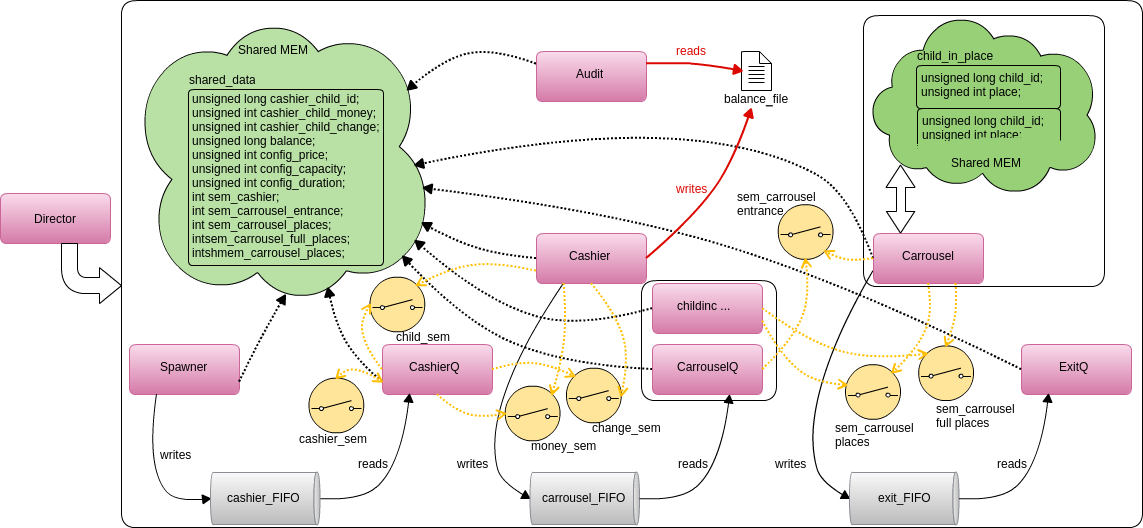
\includegraphics[scale=0.52,angle=90]{general_idea.png}
    \end{center}
 \end{figure}

\clearpage

\begin{figure}
	\subsection{Diagrama de clases}

	\begin{center}
        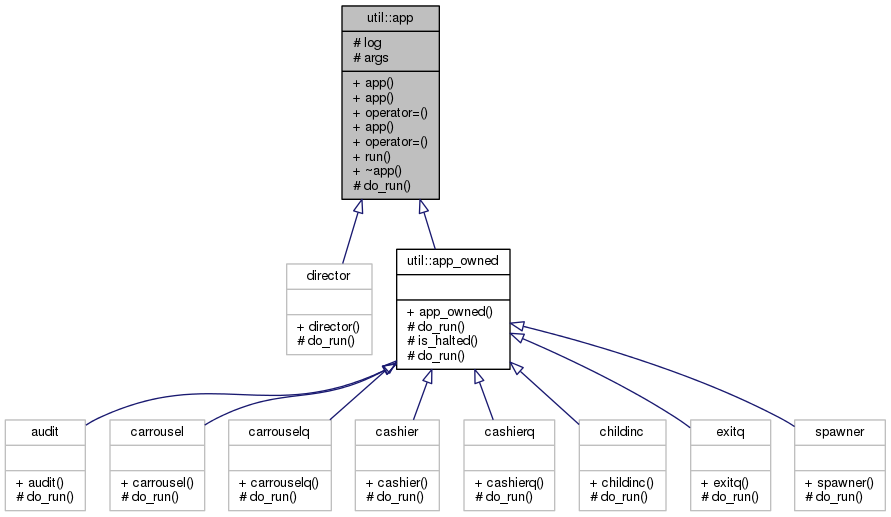
\includegraphics[scale=0.7,angle=90]{class_app.png}
    \end{center}
 \end{figure}


\clearpage

    \subsection{Diagramas de transición de estados}
	\subsubsection{Niño}
	\begin{center}
        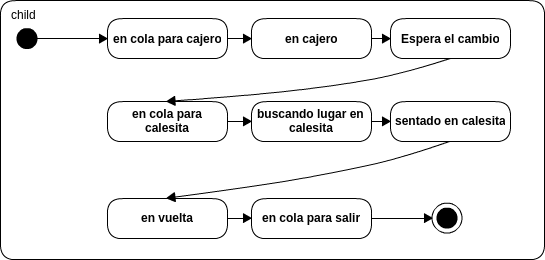
\includegraphics[scale=0.7]{chicos.png}
    \end{center}
    
    \subsubsection{Director}
    \begin{center}
        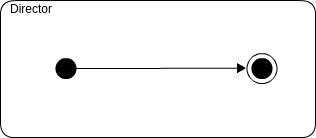
\includegraphics[scale=0.7]{director.png}
    \end{center}
    
	\subsubsection{Calesita}
    \begin{center}
        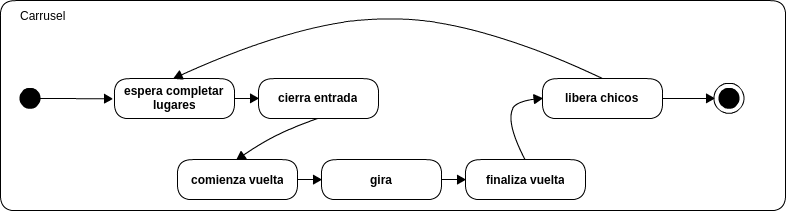
\includegraphics[scale=0.6]{calesita.png}
    \end{center}

	\subsubsection{Cajero}
	\begin{center}
        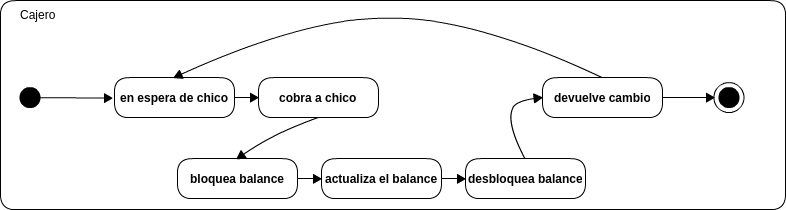
\includegraphics[scale=0.6]{cajero.png}
    \end{center}
    
	\subsubsection{Auditor}
    \begin{center}
        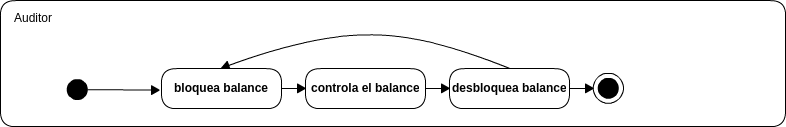
\includegraphics[scale=0.6]{auditor.png}
    \end{center}


\clearpage
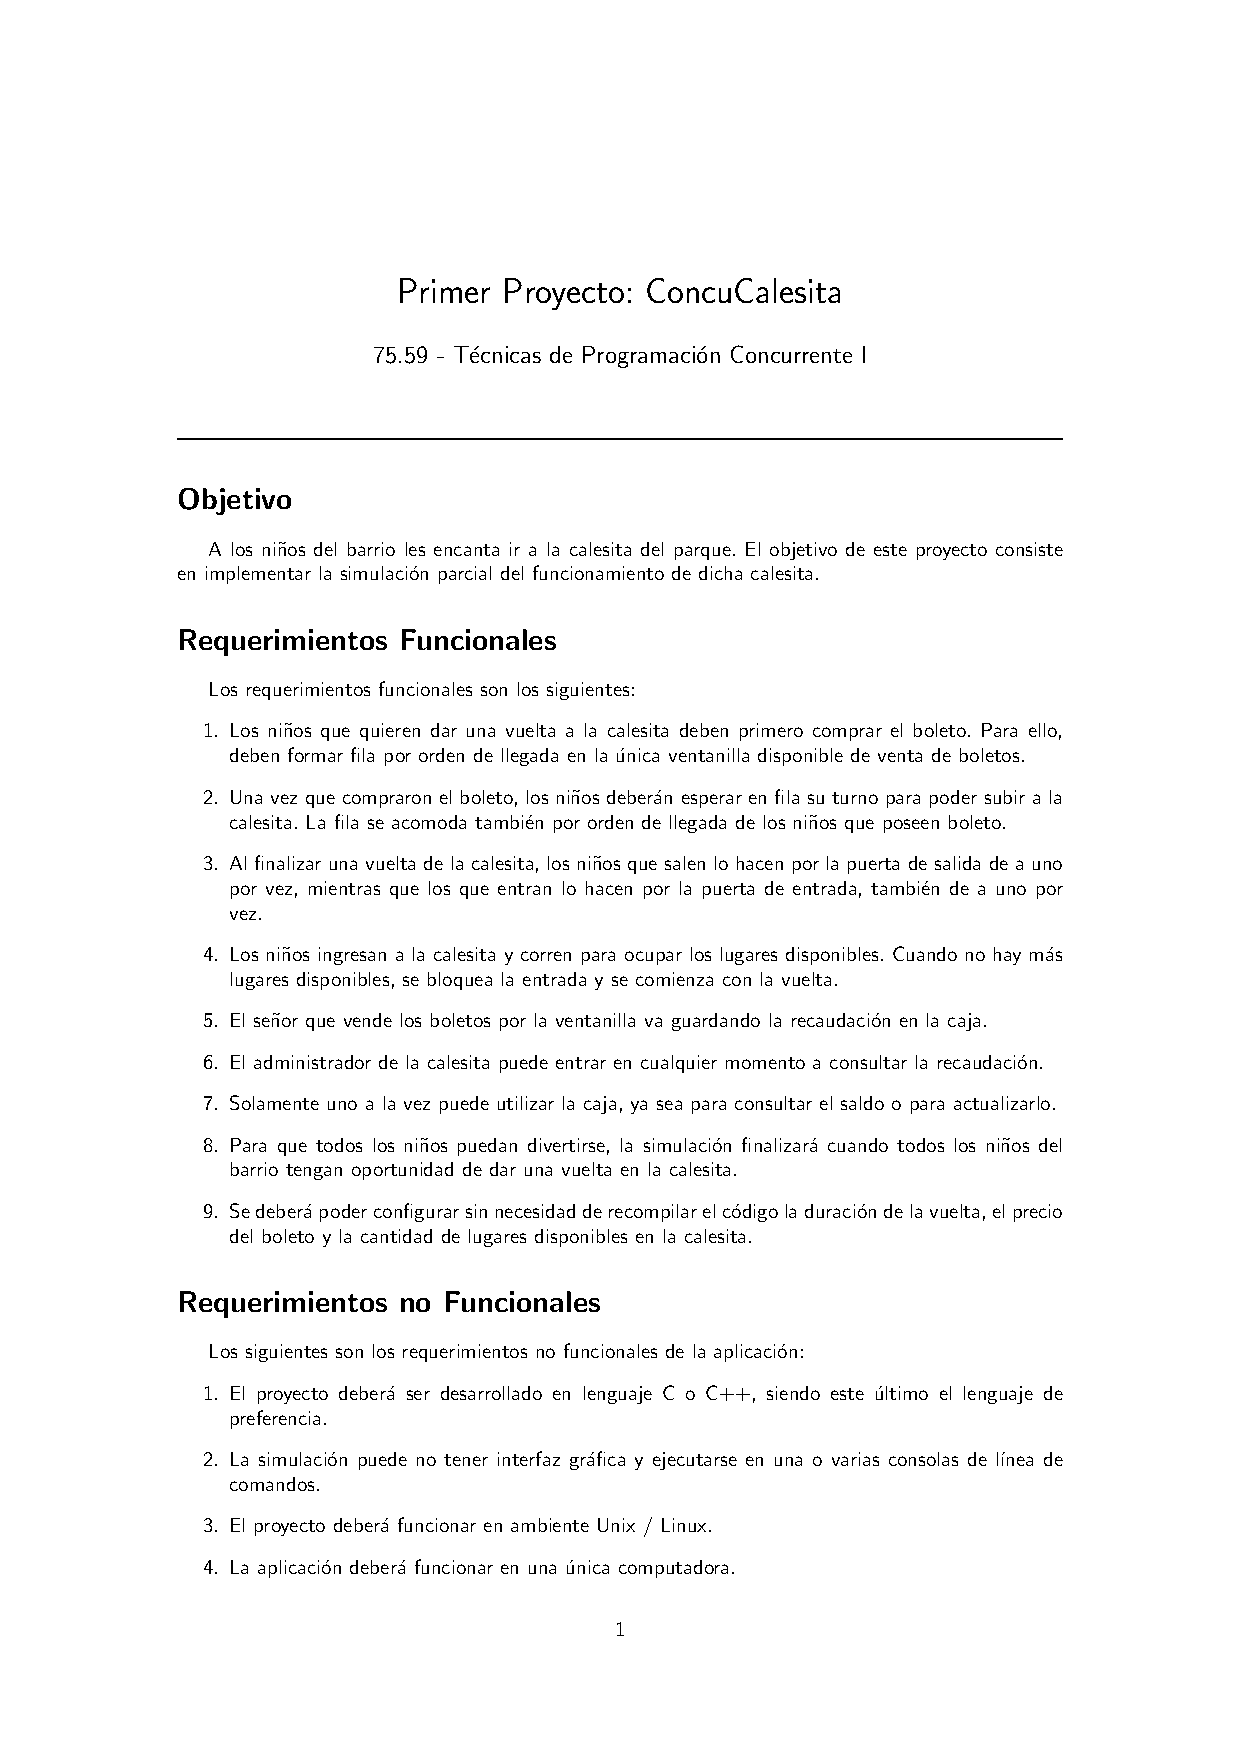
\includepdf[pages={-}]{enunciado.pdf}

\end{document}